\documentclass[11pt]{article}
\usepackage[a4paper,margin=2.5cm]{geometry}
\usepackage{times}
\usepackage{booktabs}
\usepackage{amsmath}
\usepackage{amssymb}
\usepackage{hyperref}
\usepackage{url}
\usepackage{parskip}
\usepackage{caption}
\usepackage{tikz}
\usetikzlibrary{shapes.geometric,arrows}
\usepackage{pgfplots}
\usepgfplotslibrary{groupplots}
\pgfplotsset{compat=1.18}
\usepackage{listings}
\lstdefinestyle{src}{basicstyle=\ttfamily\scriptsize\linespread{0.90}\selectfont, breaklines=true,
  breakindent=0pt, columns=fullflexible, keepspaces=true, frame=none,
  aboveskip=4pt, belowskip=4pt, xleftmargin=0pt, showstringspaces=false,
  escapeinside={(*@}{@*)}}
\emergencystretch=3em
\title{Autoresearch Loops:\\A Causal Study of the Instruction File}
\author{Christian Block\\\small Research project with Prof.\ Ramesh}
\date{\today}
\begin{document}
\maketitle

\begin{abstract}
An autoresearch loop is a system in which a language model proposes, executes and interprets experiments without a human in the loop. In the form popularized by Karpathy's \texttt{autoresearch}, the whole experimental procedure is written in English in a single instruction file, \texttt{program.md}, which therefore acts as the controller of the system. Existing work evaluates such loops end to end: it can report that a loop worked, but not which part of its instruction file was responsible. This thesis treats the instruction file as a configuration vector. Five components of \texttt{program.md} are each written at two levels, all $2^5 = 32$ combinations are generated and executed against a real executor on two tabular classification tasks with twenty replicates each, giving $1{,}280$ runs, and four behavioral metrics read from the structured transcripts are regressed on an orthogonal $\pm 1$ coding of the components with a dataset fixed effect. Because the configurations are constructed rather than observed, the coefficients admit a causal reading, and because the factorial is complete, the independence of the components can be tested rather than assumed. The results show that the components determine the process of the search rather than its outcome. The reporting style has the largest effect in the design and reduces the wasted trial ratio from $0.106$ to $0.031$; almost every wasted trial is a proposal that names a hyperparameter outside the executor's whitelist, and not a single reply in the study was malformed. The stopping rule is the only component with an effect on either outcome metric, and its effect on the gain over default is smaller than the difference between the two datasets. Three of forty two-way interactions survive adjustment, all on the wasted trial ratio and all involving the reporting style, so the components can be treated as additive. The findings are conditional on one agent model and one wording per level, and the method, rather than the particular components varied, is the contribution of this thesis.
\end{abstract}

\section{Introduction}
\label{sec:intro}

\subsection{Background}

In an autoresearch loop, the experimentation itself is performed by a language model. The model is given a goal, a body of code it may edit, and an executor that runs a trial and returns a scalar result. From that point it proceeds autonomously: it proposes a change, executes it, reads the outcome, decides what to attempt next, and repeats until the budget is exhausted. The current meaning of the term was fixed by Karpathy's \texttt{autoresearch} \cite{Karpathy2026autoresearch}, which appeared in March 2026 and has since been forked several thousand times.

The architecture is a contract between three files, each with a single owner. \texttt{prepare.py} prepares the data and defines the score; it is modified by no one, so that every experiment is scored identically. \texttt{train.py} contains the model and the training loop and is edited only by the agent, while \texttt{program.md} contains the instructions and is edited only by the human. In Karpathy's original setting each candidate is allocated five minutes of wall-clock time and yields a single number, validation bits per byte, so that trials are equally costly and directly comparable \cite{Tuychiev2026guide}. Progress is enforced through version control: a change is committed and trained, the commit is retained if the score improved, and otherwise reverted by \texttt{git reset} \cite{Tuychiev2026guide}. The repository only ever advances.

What the system does not contain is orchestration code. There is neither a scheduler nor a driver program: the nine-step experiment cycle exists only as English prose within \texttt{program.md}, and the model itself is the execution layer. \texttt{program.md} is therefore not configuration supplied to a controller; it \emph{is} the controller. This observation is the starting point of the present work.

\subsection{Motivation and Research Objective}

Such loops demonstrably function, but the reasons for their behavior remain unknown. The AI Scientist \cite{Lu2024aiscientist} and Coscientist \cite{Boiko2023coscientist} are evaluated end to end, on whether the pipeline produced an acceptable artifact, and benchmarks such as MLAgentBench \cite{Huang2024mlagentbench} report success rates across task suites. Industrial reports take the same form. An autoresearch run against a production template engine reduced parse-and-render time by $53\%$ over approximately one hundred and twenty experiments and ninety-three commits; its own author considered the gain probably overfitted, and the change was never merged \cite{Lutke2026liquid}. The system had produced a large, real and measurable improvement, and the people closest to it could not decide whether to trust it. Such evidence establishes that a loop can work; it does not establish which part of the instruction file was responsible.

The obstacle to such an attribution is confounding. An instruction file settles several matters simultaneously: what counts as success, how widely the agent may search, when it must stop, how it must report, and where effort should be concentrated. When two differently worded files are compared, every sentence differs, and no individual effect is identified. Work on prompt sensitivity sharpens the problem further. Formatting choices that preserve meaning can shift accuracy by as much as 76 points \cite{Sclar2024formatspread}, whereas models sometimes perform equally well on instructions that are irrelevant or actively misleading \cite{Webson2022prompts}. Wording evidently matters, but inspection of the wording does not reveal how.

Establishing how is an empirical problem, and this thesis addresses it experimentally. The instruction file is treated not as prose but as a configuration vector. Five components of \texttt{program.md} are each written at two levels, and all $2^5 = 32$ combinations are generated and executed against a real executor, which separates the effect of each component instead of assuming it. The contribution is a method rather than an architecture: the aim is not to propose a superior autoresearch loop, but to establish what an existing one is responding to.

The scope is deliberately narrow. No comparison is drawn between the loop and a human researcher, and neither a human baseline nor an external standard of good research practice is invoked. Every comparison is made between two configurations of the same system. The following research questions are raised:

\begin{enumerate}
\item[\textbf{RQ1}] Which components of \texttt{program.md} causally determine which aspects of the loop's research \emph{process}, and how large is each effect?
\item[\textbf{RQ2}] Do the components act independently of one another, or does the effect of one depend on the level of another?
\end{enumerate}

\subsection{Thesis Structure}

This thesis is organized into four sections. Following this introduction, Section~\ref{sec:background} describes the loop under study, shows how its instruction file is turned into a configuration vector, and explains why executing every configuration identifies the effect of each component. Section~\ref{sec:eval} presents the experimental setup, the metrics and the regression model, followed by the results, their discussion and the limitations of the study. Section~\ref{sec:conclusion} concludes the thesis by summarizing the findings and proposing directions for future work. Appendix~\ref{app:files} reproduces the three files the loop runs on, including the complete specification from which every instruction file of the study can be reconstructed.


\section{Background}
\label{sec:background}

This section gives the necessary background for the experiments. It first describes the loop that is examined and the role of the instruction file within it, then introduces the configuration space, and finally explains why constructing and executing every configuration allows the effect of each component to be read off directly.

\subsection{The Loop under Study}

The loop examined here follows the protocol described above, subject to one narrowing: the search space is a hyperparameter space rather than arbitrary code, so that the instruction file remains the only free variable. The file is supplied once as the system message and is not modified thereafter. The model then alternates between two moves, each expressed as a single JSON object. A \texttt{propose} carries a hypothesis, a model family and a set of hyperparameter values, whereas an \texttt{interpret} carries a reading of the most recent measurement together with a decision to continue or to stop.

Execution is performed by the harness, which validates each proposal and fits the estimator using scikit-learn. The validation consists of two checks: the harness parses the reply and checks that it has the required shape, and \texttt{train.py} checks the proposed hyperparameters against a fixed whitelist before any estimator is built. The whitelist is the boundary of the search space. It is not stated in \texttt{program.md}, which tells the agent only that it may choose the hyperparameters; a proposal outside it is answered with the names of the offending hyperparameters, so that the boundary is something the loop discovers by having a proposal rejected. Either way a rejected proposal is logged as an attempt, costs a turn, and does not cost an experiment. The model never computes a number; it selects what is computed and reads the result. Every value in a transcript can therefore be traced to one of two origins: it was produced by the executor, in which case it is a fact about the task, or by the model, in which case it is a fact about the loop's behavior. A run ends on the model's own stop decision, on the eighth executed experiment, or on the fourth rejected or malformed reply, whichever comes first; the two caps belong to the harness, not to the treatment. Figure~\ref{fig:loop} shows the resulting control flow.

\begin{figure}[t]
\centering
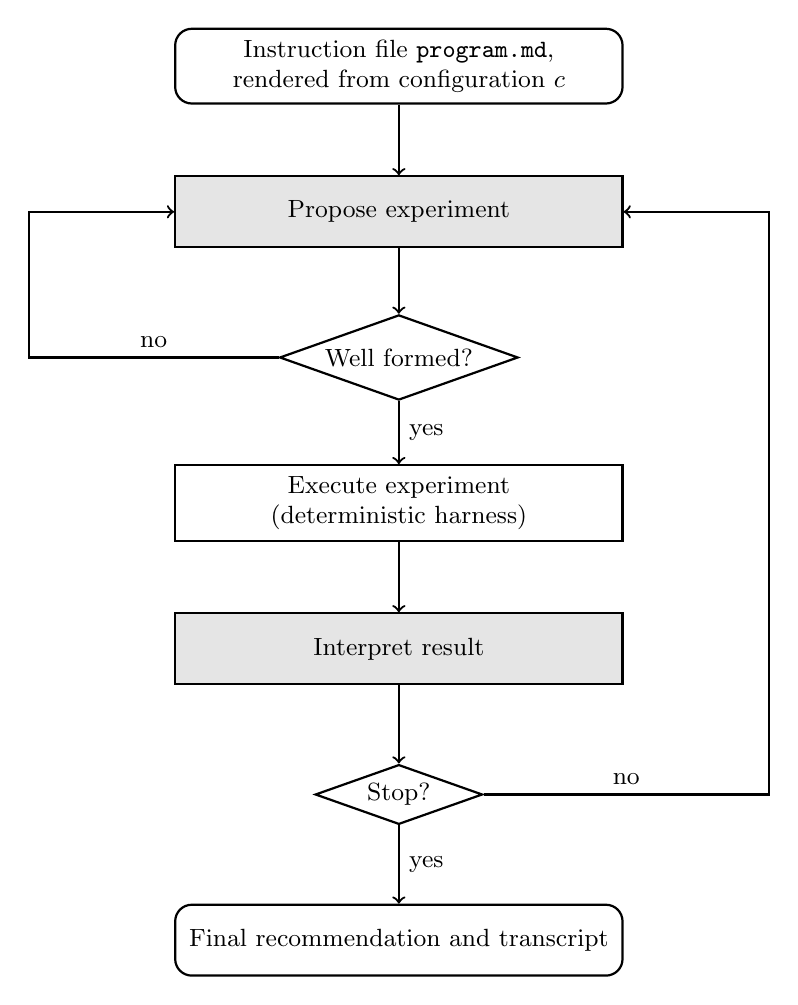
\begin{tikzpicture}[
  font=\small,
  proc/.style={rectangle, draw, thick, text width=5.4cm, align=center,
               minimum height=0.9cm, inner sep=4pt},
  llm/.style={proc, fill=gray!20},
  term/.style={rectangle, draw, thick, rounded corners=6pt, text width=5.4cm,
               align=center, minimum height=0.9cm, inner sep=4pt},
  dec/.style={diamond, draw, thick, aspect=2.8, inner sep=2pt, align=center},
  flow/.style={->, thick}
]
\node[term] (prog) at (0,0)      {Instruction file \texttt{program.md},\\rendered from configuration $c$};
\node[llm]  (prop) at (0,-1.85)  {Propose experiment};
\node[dec]  (val)  at (0,-3.7)   {Well formed?};
\node[proc] (exec) at (0,-5.55)  {Execute experiment\\(deterministic harness)};
\node[llm]  (intp) at (0,-7.4)   {Interpret result};
\node[dec]  (stop) at (0,-9.25)  {Stop?};
\node[term] (rep)  at (0,-11.1)  {Final recommendation and transcript};
\draw[flow] (prog) -- (prop);
\draw[flow] (prop) -- (val);
\draw[flow] (val)  -- node[right]{yes} (exec);
\draw[flow] (exec) -- (intp);
\draw[flow] (intp) -- (stop);
\draw[flow] (stop) -- node[right]{yes} (rep);
\draw[flow] (val.west)  -- node[above]{no} (-4.7,-3.7)  |- (prop.west);
\draw[flow] (stop.east) -- node[above]{no} (4.7,-9.25)  |- (prop.east);
\end{tikzpicture}
\caption{Control flow of one run. Shaded boxes are language-model calls. The unshaded box is deterministic, so every number the loop reasons about was measured and not generated. The validity check combines two checks in the code: the harness parses the reply and checks its shape, and \texttt{train.py} checks the whitelist before any estimator is fitted. A proposal that fails either check goes back to the proposal step; it is logged as an attempt, which is what the wasted trial ratio counts, and costs a turn but not an experiment. A run ends on the model's stop decision, on eight executed experiments, or on four rejected or malformed replies, whichever comes first.}
\label{fig:loop}
\end{figure}

\subsection{The Instruction File as a Configuration}

Every instruction file is generated from a single template. The fixed part specifies the research question, the executor interface and the JSON response format, and is byte-identical across all thirty-two files of a task. The variable part consists of five paragraphs, each written at one of two levels; these five slots constitute the independent variables, and nothing else in the file varies. A file is described completely by
\[
c = (c_1,\ldots,c_5), \qquad c_i \in \{0,1\},
\]
where the slots are taken in the order metric, breadth, stopping rule, output format and emphasis, yielding $2^5 = 32$ files. Concretely, $c = (1,0,1,1,0)$ is the file \texttt{M1-B0-S1-O1-E0}: the level-1 paragraph in the evaluation slot, level 0 in breadth, level 1 in stopping, level 1 in reporting and level 0 in emphasis. Its neighbor \texttt{M1-B0-S1-O0-E0} is the same file with one paragraph exchanged and nothing else changed, and the remaining thirty files are the other combinations.

Table~\ref{tab:axes} lists the levels. These categories were not invented for this study: a production \texttt{program.md} hardcodes the baseline to be exceeded, specifies how failures are to be handled, fixes a reporting discipline and imposes a parsimony rule \cite{Tuychiev2026guide}, and the five components below are drawn from those categories. One of them deserves a remark, because its role in the loop is easily underestimated. The loop carries no state other than its own transcript: what the model wrote in the hypothesis and interpretation fields of the previous turns is the only thing it can read back before proposing the next experiment. The reporting style $O$ therefore governs how much of the loop's reasoning is written down and made available to itself.

\begin{table}[t]
\centering
\small
\setlength{\tabcolsep}{4pt}
\caption{The five varied components of \texttt{program.md}. A configuration is one choice of level per row. The last column gives the token count of each level's paragraph, level $0$ / level $1$; the levels are not length-matched, and the consequences are discussed in the text.}
\label{tab:axes}
\begin{tabular}{@{}p{0.8cm}p{2.0cm}p{4.3cm}p{4.3cm}r@{}}
\toprule
Code & Component & Level $0$ & Level $1$ & Tokens \\
\midrule
$M$ & Evaluation criterion & Success left undefined; the loop judges quality as it sees fit. & Success defined as five-fold cross-validated accuracy, with the across-fold standard deviation used only to break ties. & 10 / 56 \\
$B$ & Search breadth & Commit to one model family for the session. & Compare both families within a session and vary several hyperparameters at once. & 32 / 26 \\
$S$ & Stopping rule & Fixed budget of exactly three experiments. & Adaptive budget of up to eight, halted when an experiment fails to improve by more than $0.002$. & 32 / 59 \\
$O$ & Reporting style & Terse: the action taken and the numbers involved. & Full sentences stating hypothesis, expectation and interpretation. & 20 / 34 \\
$E$ & Search emphasis & Explore first: several different configurations before refining any. & Exploit first: refine a promising configuration immediately. & 24 / 32 \\
\bottomrule
\end{tabular}
\end{table}

The ten paragraphs were written by a language model distinct from the agent, from fixed meta-prompts, then frozen and reused verbatim; they are reproduced in full in Appendix~\ref{app:levels}. This procedure is a control. Had the paragraphs been composed by the author, the wording of every treatment would have constituted a free parameter confounded with the author's own stylistic habits, and no measured effect could have been separated from it. The meta-prompts themselves were not preserved, so the paragraphs can be inspected and reused but not regenerated.

Two properties that such a treatment set would ideally have do not hold here, and both are visible in Appendix~\ref{app:levels}. First, the two levels of a slot are not matched in length: the token counts, given in Table~\ref{tab:axes}, differ by between a fifth and a factor of five, the extreme being the evaluation criterion, whose level-0 paragraph is a single sentence and whose level-1 paragraph is three. Paragraph length is therefore not held constant across a level switch, and could in principle stand in for the component itself. It does not appear to do so. Across the thirty-two files the total length of the five treatment paragraphs spans $112$ to $213$ tokens, and over that range it correlates with the wasted trial ratio at $r=-0.05$; across the five slots the length difference between levels is essentially uncorrelated with the size of the effect that slot produces on that metric ($r=0.23$), and the two largest effects belong to $O$ and $B$, whose levels differ by $+14$ and $-6$ tokens respectively, while the largest length difference, $+46$ tokens on $M$, produces the smallest of the four significant effects. Length does not order the results.

Second, one paragraph refers to another slot. The stopping rule at level 1 instructs the loop to stop when an experiment fails to improve \emph{the evaluation metric (defined above)} by more than $0.002$, and what is defined above is slot $M$. In the sixteen configurations with $M=0$, where the loop is told to judge quality as it sees fit, the adaptive rule therefore names a quantity that the file has deliberately left open, and $S=1$ is to that extent underspecified in half the design. This is a defect in the treatment set rather than in the estimator: $M$ and $S$ remain orthogonal by construction, and their interaction is the smallest term in the design on the metric where both act ($-0.004$ on the wasted trial ratio, adj.\ $p=0.54$), so the dependency did not produce a detectable distortion. Its consequence is for the compliance figure rather than for the coefficients, and is taken up in Section~\ref{sec:results}.

\subsection{Configuration Change as Intervention}

The configurations are constructed rather than observed: for each of the thirty-two values of $c$ the corresponding file is generated and executed. In observational prompt data the components would be correlated, since an author who writes a precise success criterion is also likely to write a careful stopping rule. Construction breaks that correlation. Across the thirty-two files, each component is at level 1 in exactly sixteen, and within each half the remaining four components remain balanced. The difference in mean outcome between runs with $c_i=1$ and runs with $c_i=0$ therefore cannot be produced by any other component. Confounding is eliminated by the design itself, without any statistical adjustment.

Executing the complete space yields more than the five main effects. Given all thirty-two files, every pairwise interaction is estimated separately from every main effect, so that the independence of the components becomes a question that can be answered from the data. A design covering only part of the space must instead assume an answer, since the runs required to distinguish a main effect from an interaction are precisely those it omits. Thirty-two cells is the cost of avoiding that assumption, and at this scale the cost is acceptable. This is what makes RQ2 testable.


\section{Experiment Setup and Results}
\label{sec:eval}

This section presents the experimental design and the results. It first describes the tasks, the executor and the baseline, the variables that are held fixed, and the size of the design. It then defines the four dependent variables and the regression model, before presenting the results, discussing them, and stating the limitations of the study. All experiments were implemented in Python; the files the loop runs on are reproduced in the appendices.

\subsection{Tasks, Executor and Baseline}

Every configuration is executed against two canonical tabular classification datasets, selected to differ in size, dimensionality and number of classes: Breast Cancer Wisconsin ($569 \times 30$, two classes) and Wine ($178 \times 13$, three classes). Each employs a single stratified $70/30$ partition, fixed with the same seed throughout. The loop may select either \texttt{RandomForestClassifier} or \texttt{GradientBoostingClassifier} under a fixed hyperparameter whitelist, that is, the set of hyperparameters the agent is allowed to name for each family; the whitelist is given in Appendix~\ref{app:train}, and anything outside it is rejected before an estimator is built. Whatever a configuration's evaluation paragraph emphasizes, the executor returns an identical record in every case: five-fold cross-validated accuracy, its across-fold standard deviation, and held-out validation accuracy. The instruction file alters what the loop attends to; it does not alter what is measured.

A single reference quantity is computed per dataset before any run, by a procedure involving no language model. The quantity $a_0(d)$ is the accuracy of a default-hyperparameter fit, taken as the better of the two model families, and every run is measured against it. It costs exactly two fits per dataset, one per family with scikit-learn's own defaults, which keeps the reference inexpensive and excludes any estimated quantity from the measurement. On both datasets the better family is the random forest, with $a_0 = 0.9598$ on Breast Cancer and $a_0 = 0.9600$ on Wine on the cross-validated scale.

One limitation of the task suite follows from this procedure. The 54-instance validation split of Wine is classified perfectly by default hyperparameters, so that $a_0$ equals $1.0$ on the validation scale and no run can improve upon it there. On that task the gain is measured on the cross-validated scale alone. This is a property of the task, not of the metric.

\subsection{Control of Non-Treatment Variation}

The following are held fixed and so cannot explain any measured effect: the agent model, pinned to the dated snapshot \texttt{gpt-4o-mini-2024-07-18} instead of a moving alias; the decoding temperature, fixed at $0.7$ for every run; the partition and its seed; the executor and its whitelist; the fixed part of the template; the response format; and the two harness caps of eight executed experiments and four rejected or malformed replies per run. Runs are separate conversations, so nothing carries over between them.

Sampling noise is treated differently: it is controlled rather than eliminated. Every run passes an explicit sampling seed to the model interface, so that any run can be regenerated exactly, and every cell draws from the same seed list, so that the draws cannot favor one configuration. Greedy decoding at temperature zero would be inappropriate here, since run-to-run variance is the error term against which every coefficient below is tested; a deterministic loop would drive that variance to zero and with it every standard error, leaving point estimates and no way to say whether any of them is distinguishable from noise. The temperature is therefore held constant and strictly above zero, which makes it a controlled constant rather than an eliminated one. When a run fails to produce a valid experiment it is repeated with a fresh seed until the cell contains exactly $R$ completed runs, so that balance is preserved by construction. Nine runs required such a replacement, four of them at the second attempt, and the study drew twenty-eight distinct seeds rather than twenty. All nine fall in two of the sixty-four cells, \texttt{M0-B0-S1-O0-E1} and \texttt{M0-B0-S1-O1-E0} on Breast Cancer, which therefore draw from a seed set differing from the other sixty-two in three and six of their twenty replicates. Both are adaptive-budget cells, which execute more experiments per run and so have more occasions to fail; every cell still holds exactly twenty completed runs, so the design remains balanced.

\subsection{Design and Budget}

The design is the complete $2^5$ factorial crossed with the task suite and replicated $R$ times, giving $N = 2^5 \cdot D \cdot R$ runs. With $D=2$ and $R=20$, this yields $N=1{,}280$ runs in 64 cells of 20. The replicate count was not chosen for convenience: it fixes the smallest detectable level switch at $0.22\,\sigma$ per dataset, where $\sigma$ denotes the run-to-run standard deviation of whichever metric is being fitted. Of the $1{,}280$ runs, $1{,}278$ terminated on the model's own stop decision and two on the cap of eight experiments; none reached the cap on rejected or malformed replies. The study issued approximately $9{,}900$ model calls and $4{,}768$ estimator fits, the latter consuming $74$ minutes of executor time in total, so the cost of the design is dominated by the model interface rather than by the machine learning.

\subsection{Metrics}

Four dependent variables are read directly off the structured transcript. No evaluation framework, scoring library or judge model is involved, since each is a difference in accuracy, a proportion of the proposals, or a count of executor calls, so nothing in the measurement can drift with the instruction being tested. Two of the four describe what a run achieved and two describe what the search cost, and the results turn on this distinction.

\paragraph{Measurement window.} The stopping rule determines how many experiments a run performs, and every metric below aggregates over those experiments. A best score improves with the number of trials for reasons unrelated to the quality of the search, and a ratio computed over more proposals is estimated more precisely. Every metric is therefore computed over the first three experiments, this being the number performed at the fixed-budget level and hence the number available in every run. Complete-run values are reported separately in Section~\ref{sec:discussion}.

\paragraph{Outcome metrics.} The \emph{gain over default} is the difference between the score of the configuration finally recommended by the run and $a_0(d)$. It answers the primary question concerning the result, namely whether the tuning achieved anything that untuned defaults would not have given. A negative value indicates that the run terminated on a configuration inferior to untuned defaults. Where a run named a final configuration that it had executed, which was the case in $1{,}028$ of the $1{,}280$ runs, that configuration's score is used; otherwise the best executed score stands in, and the transcript records which basis applied.

The \emph{improvement rate} is the proportion of executed trials whose score is strictly higher than the best score observed earlier in the same run. The first trial has nothing earlier to beat and so can never count as an improvement, while the denominator remains every executed trial; within the three-experiment window the metric is therefore bounded above by $2/3$, and that bound is attained. A run of three trials with no improvement after the first is close to guessing, whereas a high rate is evidence that the interpret step is genuinely informing the next proposal.

\paragraph{Efficiency metrics.} The \emph{wasted trial ratio} is the number of proposals rejected before execution, whether malformed, of the wrong shape or invalid against the whitelist, together with the number that exactly duplicate an earlier proposal in the same run, divided by the total number of proposals attempted. Both failure modes consume a turn without yielding a measurement.

The \emph{cost to best} is the number of executor calls made up to and including the call that produced the highest score of the run, taking the earliest such call on ties. Exploration after that point does not count. Since every executed trial consumes the same fixed budget, this is the computation spent to reach the result.

\paragraph{A qualification.} The evaluation-criterion component at level 1 names cross-validated accuracy, which is the scale on which the gain over default is computed, so part of any effect that component shows is the treatment agreeing with the instrument. For Breast Cancer the gain on held-out validation accuracy is therefore reported as a robustness check, and an effect is claimed for that component only where both scales agree. Wine allows no such check, for the reason given above.

\subsection{Regression Model and Inference}

Each component is coded as an indicator variable
\begin{equation}
X_i = \begin{cases} +1 & \text{if component } i \text{ is at level } 1,\\ -1 & \text{if at level } 0,\end{cases}
\qquad i = 1,\ldots,5,
\label{eq:coding}
\end{equation}
and the outcome of one run is modeled as
\begin{equation}
Y \;=\; \beta_0 + \sum_{i=1}^{5}\beta_i X_i + \sum_{j=2}^{D}\gamma_j D_j + \varepsilon ,
\label{eq:regression}
\end{equation}
where $D_j$ indicates that the run was made on dataset $j$, the first dataset serving as the reference level. The $\gamma_j$ are dataset fixed effects: they absorb the inherent difficulty of each task, its headroom above $a_0(d)$ and its response to the whitelist, which would otherwise sit in the residual and inflate every standard error. Because the factorial is crossed with the task suite, each $X_i$ is orthogonal to every $D_j$ by construction, so the $\hat\beta_i$ are within-task effects of the components and are not contaminated by which tasks happen to be easy. Here $\beta_0$ denotes the mean across configurations on the reference dataset, $\beta_i$ the effect of component $i$, and $\varepsilon$ run-to-run error. Under the coding of equation~\eqref{eq:coding}, each $X_i$ assumes each value equally often and independently of the remainder, so that $\hat\beta_i$ does not shift when another component enters or leaves the model, and $2\beta_i$ is the average change in $Y$ produced by switching component $i$; it is $2\hat\beta_i$ that is reported throughout. Since all thirty-two configurations are executed, the interaction model is obtained at no additional cost,
\begin{equation}
Y \;=\; \beta_0 + \sum_{i=1}^{5}\beta_i X_i + \sum_{1\le i<j\le 5}\beta_{ij}X_iX_j + \sum_{j=2}^{D}\gamma_j D_j + \varepsilon ,
\label{eq:interaction}
\end{equation}
which is how RQ2 is tested.

Estimation proceeds by ordinary least squares on the individual runs rather than on the cell means. Because the design is balanced the coefficients are identical under either choice, while the error term now reflects run-to-run scatter. Balance would likewise equalize the standard errors if the error variance were constant, which it is not: the stopping rule fixes the experiment count at one level and frees it at the other, so within-cell variance differs systematically between the two halves of the design. Heteroskedasticity-consistent (HC3) standard errors are therefore used throughout, and the wasted trial ratio and the improvement rate are fitted on their natural scale, both being proportions. Multiplicity is handled by Benjamini--Hochberg adjustment, with the family taken as the treatment coefficients of one model on one metric; the dataset fixed effects are controls, not hypotheses, and are excluded from the family. For equation~\eqref{eq:regression} the family is the five main effects, and for equation~\eqref{eq:interaction} it is the fifteen treatment coefficients of that model, of which ten are the pairwise terms reported below.

\subsection{Results}
\label{sec:results}

\paragraph{What the runs did.} Before the estimates are presented, Table~\ref{tab:descriptives} describes the $1{,}280$ runs themselves. In total the loop attempted $5{,}140$ proposals, of which $4{,}768$ were executed and $372$ were rejected, and only five proposals in the whole study exactly duplicated an earlier one. The composition of the rejections is informative. Not one of the $5{,}140$ replies was malformed JSON or of the wrong shape: $369$ of the $372$ rejections were whitelist violations, $365$ of them on the random forest and four on gradient boosting, and the remaining three were estimator fits that failed. The hyperparameters the loop reached for were legitimate scikit-learn arguments that the whitelist does not admit, above all \texttt{min\_samples\_split} on the random forest, which accounts for $290$ of the $369$ violations, followed by \texttt{random\_state} with $71$. In this study the wasted trial ratio is therefore, almost entirely, the rate at which the loop names a hyperparameter outside an interface it has not been shown.

\begin{table}[t]
\centering
\small
\caption{Run-level descriptive statistics over the complete runs. Upper panel: per-run quantities across all $1{,}280$ runs. Lower panel: per-run means by level of the stopping rule $S$ and the reporting style $O$. Study totals: $5{,}140$ proposals attempted, $4{,}768$ experiments executed, $372$ proposals rejected, 5 duplicates.}
\label{tab:descriptives}
\begin{tabular}{lrrr}
\toprule
Per run & Mean & Median & Max \\
\midrule
Proposals attempted    & $4.02$  & $3$ & $9$ \\
Experiments executed   & $3.73$  & $3$ & $8$ \\
Proposals rejected     & $0.29$  & $0$ & $2$ \\
Duplicate proposals    & $0.004$ & $0$ & $1$ \\
Executor calls to best & $1.71$  & $1$ & $7$ \\
\multicolumn{4}{l}{\footnotesize\itshape (complete runs; within the three-experiment window the maximum is 3)} \\
\midrule
Per run (mean) & $S=0$ fixed & $S=1$ adaptive & \\
\midrule
Experiments executed   & $2.88$ & $4.57$ & \\
Proposals rejected     & $0.17$ & $0.41$ & \\
Experiments after best & $1.30$ & $2.73$ & \\
\midrule
Per run (mean) & $O=0$ terse & $O=1$ full sentences & \\
\midrule
Experiments executed   & $3.76$ & $3.69$ & \\
Proposals rejected     & $0.43$ & $0.15$ & \\
\bottomrule
\end{tabular}
\end{table}

Most runs reached their best score almost at once. The best score arrived on the first executor call in $720$ runs ($56.2\%$), on the second in $291$ ($22.7\%$), on the third in $222$ ($17.3\%$), and on a later call in only $47$ runs ($3.7\%$); no run needed more than seven calls. Consequently $56\%$ of runs never improved on their first trial and $96.3\%$ never improved after their third. On average $2.02$ experiments per run were executed after the best had already been found, which amounts to $2{,}585$ of the $4{,}768$ executed trials, more than half of the compute in the study. On the gain over default, $40.0\%$ of runs improved on $a_0$, $39.1\%$ recommended a configuration scoring exactly $a_0$, and $20.9\%$ terminated below it.

\paragraph{Main effects.}

\begin{table}[t]
\centering
\small
\caption{Main-effect estimates $2\hat\beta_i$ per metric from equation~\eqref{eq:regression}, with heteroskedasticity-consistent standard errors and Benjamini--Hochberg adjusted $p$-values. The $\hat\gamma$ column is the fitted dataset fixed effect (Wine relative to Breast Cancer).
Stars mark adjusted $p<0.05$ ($^{*}$), $<0.01$ ($^{**}$) and $<0.001$ ($^{***}$).}
\label{tab:main}
\begin{tabular}{lrrrrrrr}
\toprule
Metric & $M$ & $B$ & $S$ & $O$ & $E$ & $\hat\gamma$ & $R^2$ \\
\midrule
Gain over default   & +0.001 & -0.001 & +0.001$^{**}$ & +0.000 & +0.000 & -0.001$^{***}$ & 0.029 \\
Wasted trial ratio  & -0.023$^{***}$ & -0.034$^{***}$ & +0.044$^{***}$ & -0.075$^{***}$ & +0.005 & -0.003 & 0.159 \\
Improvement rate    & +0.008 & -0.026$^{*}$ & +0.034$^{**}$ & +0.006 & +0.018 & -0.064$^{***}$ & 0.044 \\
Cost to best        & +0.06 & -0.02 & +0.05 & -0.01 & -0.11 & -0.20$^{***}$ & 0.025 \\
\bottomrule
\end{tabular}
\end{table}

\begin{figure}[t]
\centering
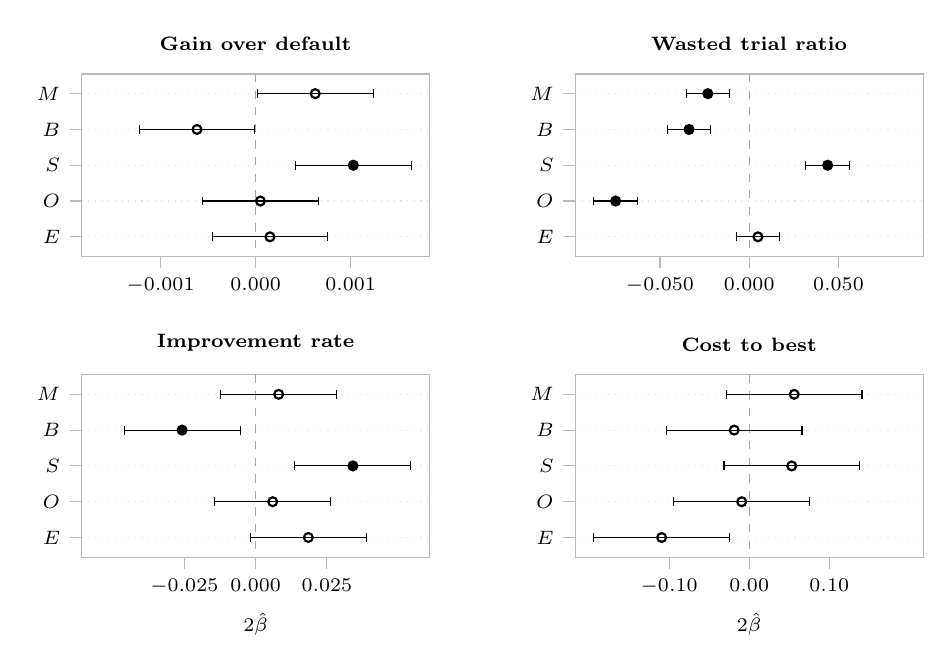
\begin{tikzpicture}[font=\scriptsize]
\begin{groupplot}[
  group style={group size=2 by 2, horizontal sep=1.85cm, vertical sep=1.5cm},
  width=6.0cm, height=3.9cm,
  y dir=reverse, ytick={1,2,3,4,5},
  yticklabels={$M$,$B$,$S$,$O$,$E$},
  ymin=0.45, ymax=5.55,
  ymajorgrids, major grid style={gray!22, dotted},
  axis line style={gray!55}, tick align=outside, tick pos=left,
  every tick/.style={gray!55},
  title style={font=\scriptsize\bfseries, yshift=-1pt},
  scaled x ticks=false,
]
\nextgroupplot[title={Gain over default}, xmin=-0.00183, xmax=0.00183,
  xtick={-0.001,0.000,0.001}, xticklabel style={/pgf/number format/fixed,
    /pgf/number format/precision=3, /pgf/number format/fixed zerofill},]
\addplot[gray!70, dashed, forget plot] coordinates {(0,0.45) (0,5.55)};
\addplot[only marks, mark=*, mark size=1.6pt, black, thick,
  error bars/.cd, x dir=both, x explicit, error bar style={black}]
  coordinates {(0.001028,3) +- (0.000609,0)};
\addplot[only marks, mark=o, mark size=1.6pt, black, thick,
  error bars/.cd, x dir=both, x explicit, error bar style={black}]
  coordinates {(0.000627,1) +- (0.000609,0) (-0.000617,2) +- (0.000609,0) (0.000050,4) +- (0.000609,0) (0.000151,5) +- (0.000609,0)};
\nextgroupplot[title={Wasted trial ratio}, xmin=-0.09746, xmax=0.09746,
  xtick={-0.050,0.000,0.050}, xticklabel style={/pgf/number format/fixed,
    /pgf/number format/precision=3, /pgf/number format/fixed zerofill},]
\addplot[gray!70, dashed, forget plot] coordinates {(0,0.45) (0,5.55)};
\addplot[only marks, mark=*, mark size=1.6pt, black, thick,
  error bars/.cd, x dir=both, x explicit, error bar style={black}]
  coordinates {(-0.023177,1) +- (0.012178,0) (-0.033698,2) +- (0.012178,0) (0.043958,3) +- (0.012178,0) (-0.074844,4) +- (0.012178,0)};
\addplot[only marks, mark=o, mark size=1.6pt, black, thick,
  error bars/.cd, x dir=both, x explicit, error bar style={black}]
  coordinates {(0.004896,5) +- (0.012178,0)};
\nextgroupplot[title={Improvement rate}, xlabel={$2\hat\beta$}, xmin=-0.06099, xmax=0.06099,
  xtick={-0.025,0.000,0.025}, xticklabel style={/pgf/number format/fixed,
    /pgf/number format/precision=3, /pgf/number format/fixed zerofill},]
\addplot[gray!70, dashed, forget plot] coordinates {(0,0.45) (0,5.55)};
\addplot[only marks, mark=*, mark size=1.6pt, black, thick,
  error bars/.cd, x dir=both, x explicit, error bar style={black}]
  coordinates {(-0.025781,2) +- (0.020340,0) (0.034115,3) +- (0.020340,0)};
\addplot[only marks, mark=o, mark size=1.6pt, black, thick,
  error bars/.cd, x dir=both, x explicit, error bar style={black}]
  coordinates {(0.008073,1) +- (0.020340,0) (0.005990,4) +- (0.020340,0) (0.018490,5) +- (0.020340,0)};
\nextgroupplot[title={Cost to best}, xlabel={$2\hat\beta$}, xmin=-0.21731, xmax=0.21731,
  xtick={-0.10,0.00,0.10}, xticklabel style={/pgf/number format/fixed,
    /pgf/number format/precision=2, /pgf/number format/fixed zerofill},]
\addplot[gray!70, dashed, forget plot] coordinates {(0,0.45) (0,5.55)};
\addplot[only marks, mark=o, mark size=1.6pt, black, thick,
  error bars/.cd, x dir=both, x explicit, error bar style={black}]
  coordinates {(0.056250,1) +- (0.084652,0) (-0.018750,2) +- (0.084652,0) (0.053125,3) +- (0.084652,0) (-0.009375,4) +- (0.084652,0) (-0.109375,5) +- (0.084652,0)};
\end{groupplot}
\end{tikzpicture}
\caption{Estimated component effects on every metric. Points are $2\hat\beta_i$ from
equation~\eqref{eq:regression}, bars are $95\%$ intervals built from
heteroskedasticity-consistent standard errors, and a filled point marks an effect that
survives Benjamini--Hochberg adjustment at $0.05$. The dataset fixed effect is in the
model, so these are within-task effects. The four panels carry independent horizontal
scales, the metrics being in different units.}
\label{fig:coefficients}
\end{figure}

Table~\ref{tab:main} gives the main-effect estimates and Figure~\ref{fig:coefficients} plots them with their intervals. It is visible that the components affect the four metrics unequally.

The wasted trial ratio is the most responsive metric. Four of the five components produce effects that survive adjustment, and the model accounts for $R^2=0.16$ of its variance. The reporting style produces the largest effect measured anywhere in the design, $2\hat\beta_O=-0.075$, corresponding to a reduction in the mean ratio from $0.106$ at level $0$ to $0.031$ at level $1$. Given the composition of the rejections described above, this is a reduction in whitelist violations: $273$ of the $369$ occurred in runs with terse reporting and $96$ in runs with full sentences. Search breadth and the evaluation criterion act in the same direction, with effects of $-0.034$ and $-0.023$. The adaptive stopping rule acts in the opposite direction, $+0.044$, raising the mean ratio from $0.046$ to $0.090$. This is consistent with its mechanism. The adaptive level raises the mean number of executed experiments from $2.88$ to $4.57$ and the mean number of rejected proposals per run from $0.17$ to $0.41$; the additional proposals do not duplicate earlier ones, of which there are only five in the study, but reach more often for a hyperparameter outside the whitelist, $260$ of the $369$ violations occurring under the adaptive rule.

The two outcome metrics, by contrast, respond to the stopping rule alone. It is the only component whose effect on the gain over default survives adjustment ($+0.001$, adj.\ $p=0.005$), and it raises the improvement rate from $0.135$ to $0.170$. Search breadth is the only other component affecting the improvement rate, at $-0.026$. No component affects the cost to best at the adjusted $0.05$ level; the largest estimate is exploit-first at $-0.11$, with adj.\ $p=0.057$. The components that determine efficiency are therefore not the components that determine outcome.

Furthermore, on two of the four metrics the dataset fixed effect is roughly twice the largest component effect. Wine reduces the improvement rate by $0.064$ and the cost to best by $0.20$ relative to Breast Cancer, both at $p<10^{-5}$, against largest component effects of $0.034$ and $0.11$ on the same metrics. Which task the loop is run on matters more for these two metrics than how the instruction file is worded, and this is exactly the variation that equation~\eqref{eq:regression} removes from the residual.

\paragraph{Interactions.} Table~\ref{tab:interactions} gives the two-way interactions. Three of the forty estimated across the four metrics survive adjustment; for the remaining thirty-seven the data provide no evidence of interaction. All three occur on the wasted trial ratio and all three involve the reporting style: $S\times O$ at $-0.031$, $B\times O$ at $+0.018$, and $O\times E$ at $-0.016$. Of these, only $S\times O$ is comparable in magnitude to a main effect, and its sign indicates complementarity rather than substitution. The cell means make the direction plain: the adaptive budget raises the mean wasted trial ratio from $0.068$ to $0.143$ when reporting is terse, but only from $0.024$ to $0.037$ when it is in full sentences, so that the additive prediction for the adaptive-and-verbose cell, $0.100$, overstates the observed $0.037$ by a factor of nearly three. Equivalently, the reduction the reporting style buys is larger under an adaptive budget ($-0.106$) than under a fixed one ($-0.043$). A generous experiment budget is expensive in wasted proposals only when the loop is also reporting tersely. The remaining two interactions are smaller and of opposite character: $B\times O$ is the substitution case, both components reducing waste and each reducing it less when the other is already at level $1$, while $O\times E$ resembles $S\times O$. Adding all ten interaction terms to the model of the wasted trial ratio raises $R^2$ only from $0.159$ to $0.192$, and the same three terms survive adjustment, with unchanged signs, when the ratio is refitted on the logit, square-root or arcsine-square-root scale, so the interaction structure is not an artifact of fitting a proportion on its natural scale. The components may therefore be treated as additive, which is the answer to RQ2, and the complete factorial is what permits the question to be tested rather than assumed.

\begin{table}[t]
\centering
\small
\caption{Two-way interaction estimates $2\hat\beta_{ij}$ from equation~\eqref{eq:interaction}, and compliance per component. The four interactions with the smallest adjusted $p$ are
shown, with adjusted $p$ given directly; compliance is reported as level $0$ / level $1$.}
\label{tab:interactions}
\begin{tabular}{lrr@{\hskip 1.2cm}lr}
\toprule
Interaction & Estimate & adj.\ $p$ & Component & Compliance \\
\midrule
$S \times O$ (wasted trial ratio) & -0.031 & 0.000 & $B$ & 0.66 / 0.82 \\
$B \times O$ (wasted trial ratio) & +0.018 & 0.009 & $S$ & 0.89 / 0.20 \\
$O \times E$ (wasted trial ratio) & -0.016 & 0.019 & $E$ & 0.88 / 0.69 \\
$M \times B$ (wasted trial ratio) & -0.010 & 0.171 & $O$ & 205 / 386 chars \\
 &  &  & $M$ & not observable \\
\bottomrule
\end{tabular}
\end{table}

\paragraph{Compliance.} An instruction is not invariably obeyed. Table~\ref{tab:interactions} therefore also reports the proportion of runs whose behavior matched the instruction given, so that a component without effect can be distinguished from one the model disregarded. Three components constrain an observable action and admit a mechanical check: $B$ by the number of model families the run proposes, $S$ by the number of experiments it performs, and $E$ by whether its second proposal refines the first, a check that is defined only for the $1{,}268$ runs with at least two experiments. Refinement is operationalized as a second proposal naming the same model family and carrying over at least one hyperparameter value from the first. This threshold matters, and is reported so that the figure below can be read against it: under the weaker reading that any second proposal in the same family counts as a refinement, exploit-first compliance rises from $0.69$ to $0.98$ and explore-first compliance falls from $0.88$ to $0.60$. $O$ constrains wording rather than action, so it is assigned a manipulation check instead, namely the mean number of characters of hypothesis and interpretation text per step. $M$ leaves no behavioral trace at all, because the executor computes the score whatever the instruction says. The manipulation check separates the two levels of the reporting style clearly: the mean quantity of model-written text per step is $205$ characters at level $0$ and $386$ at level $1$. Compliance with the remaining instructions is, however, only partial. The fixed budget is followed in $89\%$ of runs, whereas the adaptive rule is followed in only $20\%$. The stopping-rule effects reported above therefore measure the effect of offering an adaptive budget, not the effect of a loop that reliably terminates on diminishing returns. Two qualifications attach to that $20\%$. The check scores the adaptive rule against cross-validated accuracy for every run, including the half of the design where $M=0$ leaves the criterion to the loop's own judgment, so a run that stopped consistently on a criterion of its own is recorded as non-compliant. And, as Section~\ref{sec:background} notes, the level-1 stopping paragraph refers to a metric defined in slot $M$, which under $M=0$ is not defined at all. Compliance with the adaptive rule is indeed lower where the criterion is left open, $0.16$ against $0.23$ where it is specified, but it is low on both sides, so the underspecification is at most a part of the explanation. Search breadth is followed in $66\%$ of narrow runs and $82\%$ of broad runs, and exploit-first in $69\%$ of runs against $88\%$ for explore-first. All estimates in Table~\ref{tab:main} are consequently intention-to-treat estimates: they measure the effect of issuing an instruction rather than the effect of a loop that follows it, and are attenuated towards zero relative to the effect on runs that complied.

\subsection{Discussion}
\label{sec:discussion}

Taken together, the recovered effect structure is concentrated on process, and outcome is barely affected. Four of the five components move the wasted trial ratio, the largest being the reporting style at $-0.075$, which cuts the mean ratio from $0.106$ to $0.031$. The gain over default answers only to the stopping rule, and by $+0.001$ on the accuracy scale, a quantity smaller in absolute value than the $-0.0013$ contributed by the choice of dataset. Two components move the improvement rate, the stopping rule at $+0.034$ and search breadth at $-0.026$. On the cost to best nothing reaches the adjusted $0.05$ level. Among the two-way interactions only $S\times O$ ($-0.031$) is comparable in magnitude to a main effect, and its sign indicates substitution, not reinforcement.

Two conclusions follow. First, within the range of wordings tested, the instruction file determines the efficiency of the search but not the quality of the configuration returned. Requiring the model to state its reasoning removes approximately two thirds of the rejected proposals, a large and reproducible effect, whereas no component produced a comparable change in the accuracy of the recommended configuration. Second, the outcome effects are bounded by the difficulty of the task. Default hyperparameters already achieve $a_0 \approx 0.96$ on both datasets; $40.0\%$ of runs improve on that value, $39.1\%$ return it exactly and $20.9\%$ terminate below it, so the available headroom is small. The measured effects concern the efficiency with which a ceiling is approached, and say nothing about the height of that ceiling. Whether the same structure holds on tasks with greater headroom is not determined by this design.

What the wasted trial ratio measures deserves to be stated precisely, because the composition of the rejections is not what its definition might suggest. The metric was defined to capture malformed replies, whitelist violations and duplicates alike, but in the $5{,}140$ proposals of this study the first and third categories are empty for practical purposes: the agent model never failed the response format, and it consulted its transcript well enough to repeat itself only five times. What varies between configurations is how often the loop proposes a hyperparameter that scikit-learn accepts but the executor's whitelist does not, and it does so without ever having been shown the whitelist. The reporting style reduces this rate by about two thirds. This is consistent with the observation in Section~\ref{sec:background} that the transcript is the loop's only state, so that a loop which writes its hypotheses and interpretations in full has more of its own reasoning, including the executor's earlier rejection messages and its response to them, available to itself when it proposes the next experiment. The present design establishes the size of the effect, not this mechanism, and a study that disclosed the whitelist in \texttt{program.md} would be the direct test.

The measurement window also matters, and the complete-run values promised above bear this out. Over the full run the stopping rule's effect on the gain over default disappears ($-0.0001$, adj.\ $p=0.84$), while its effect on the cost to best appears ($+0.26$, adj.\ $p<0.001$), for the mechanical reason that an adaptive run executes more experiments and so can reach its best score later; exploit-first likewise lowers the complete-run cost to best by $0.17$ (adj.\ $p=0.004$). The effects on the wasted trial ratio are stable across the two windows, with the reporting style at $-0.060$ over the full run. On the complete-run gain the evaluation criterion shows $+0.0011$ (adj.\ $p=0.005$), but on the validation scale of Breast Cancer the same component is $-0.0005$ within the window (adj.\ $p=0.67$) and $-0.0010$ over the full run (adj.\ $p=0.12$). The two scales disagree in sign, which is the pattern expected when a treatment that names the instrument is measured on that instrument, and no effect of the evaluation criterion on outcome is claimed.

\subsection{Limitations}

Four boundary conditions delimit these results. Every finding is conditional on one agent model, so what has been measured is the action of instructions on a single policy, not a property of instructions in general. Each level is realized by one generated paragraph: the semantics of a component were held fixed, but neither its phrasing nor its length was varied, so the variance attributable to wording cannot be separated from the variance attributable to the architectural constraint itself. This is the limitation the treatment set bears most directly, and Section~\ref{sec:background} reports the two respects in which that set falls short of the ideal: the levels of a slot are not length-matched, and the level-1 stopping paragraph refers to the evaluation slot, which leaves it underspecified in half the design. Neither defect orders the results, but both would be removed by generating several wordings per level, and the meta-prompts that would make such a regeneration possible were not preserved. The evaluation covers two datasets, which leaves the dataset fixed effect resting on a single contrast. The search space is a small discrete set of hyperparameters rather than code. Within those bounds the study is a proof of concept, and its claim is correspondingly narrow: that editing the constraints in \texttt{program.md} has a measurable causal influence on the loop's behavior. Establishing the size and the generality of that influence is left to the wider designs these conditions leave open.


\section{Conclusion}
\label{sec:conclusion}

In an autoresearch loop, \texttt{program.md} performs the function that controller code performs in conventional software, yet it cannot be read in the manner of code. This thesis has treated it as a configuration vector. Five components of \texttt{program.md} were written at two levels each, all $2^5=32$ configurations were generated and executed against a real executor on two datasets with twenty replicates apiece, and the resulting behavior of the $1{,}280$ runs was reduced to four metrics and regressed on an orthogonal $\pm1$ coding of the components. Because the configurations were constructed rather than collected, the coefficients admit a causal reading. Because the factorial is complete, the independence of the components could be tested rather than assumed.

\subsection{Contributions}

The main contributions of this thesis are as follows.

\begin{enumerate}
\item \textbf{A method for attributing the behavior of an autoresearch loop to its instruction file.} The instruction file is partitioned into slots, each slot is written at two levels by a model distinct from the agent, the complete factorial is executed, and the effects are estimated by a regression whose orthogonal coding and dataset fixed effect follow from the design. The method is not tied to the five components varied here.
\item \textbf{An answer to RQ1.} The components determine the process, not the outcome. The reporting style produced the largest effect in the design, reducing the mean wasted trial ratio from $0.106$ to $0.031$, and search breadth and the evaluation criterion moved the same metric by $-0.034$ and $-0.023$. Almost every wasted trial was a proposal naming a hyperparameter outside an undisclosed whitelist, and none was a malformed reply. The stopping rule was the only component with an effect on either outcome metric, $+0.001$ on the gain over default and $+0.034$ on the improvement rate, and no component determined the cost to best. On two of the four metrics the dataset fixed effect exceeded every component effect, which is the reason equation~\eqref{eq:regression} controls for it.
\item \textbf{An answer to RQ2.} Thirty-seven of the forty two-way interactions show no evidence of interaction. The three that survive adjustment are all on the wasted trial ratio and all involve the reporting style, and together the ten interaction terms raise $R^2$ on that metric only from $0.159$ to $0.192$, so the components may be treated as additive.
\end{enumerate}

For tasks of this difficulty, the instruction file determines how the loop conducts its search rather than what the search returns.

\subsection{Future Work}

Any instruction file that can be partitioned into slots may be studied in the same manner, and full enumeration remains inexpensive while the number of slots is small. Four extensions are indicated by the limitations above. Sampling several wordings per level would separate a component from its phrasing, which is the most serious of those limitations, and would at the same time remove the two defects of the present treatment set by allowing length and cross-reference to be controlled across a family of wordings rather than fixed in a single one. Applying the procedure to a loop that edits code rather than hyperparameters would test it in a setting where the instruction file carries considerably more of the system's behavior. Tasks with greater headroom above their default configuration would show whether the outcome metrics remain as unresponsive as they were here, or whether their unresponsiveness was a ceiling effect. Finally, the composition of the wasted trials points to a direct follow-up: disclosing the executor's whitelist in \texttt{program.md}, or varying whether it is disclosed, would establish whether the effect of the reporting style is an effect on how the loop learns its interface, as the present results suggest, or on something else.

\begin{thebibliography}{99}

\bibitem{Lutke2026liquid}
T. L\"utke. Performance: 53\% faster parse+render, 61\% fewer allocations.
Pull request \#2056, Shopify/liquid, 2026. Produced by an autoresearch run of
approximately 120 experiments over 93 commits; unmerged at the time of writing.
\url{https://github.com/Shopify/liquid/pull/2056}.

\bibitem{Tuychiev2026guide}
B. Tuychiev. A guide to Andrej Karpathy's AutoResearch: automating ML with AI
agents. DataCamp tutorial, 23 March 2026. Secondary source; it reports the
contents of the repository's \texttt{program.md} and results log.
\url{https://www.datacamp.com/tutorial/guide-to-autoresearch}.

\bibitem{Boiko2023coscientist}
D. A. Boiko, R. MacKnight, B. Kline, and G. Gomes. Autonomous chemical research
with large language models. Nature, 624(7992):570--578, 2023.
doi:10.1038/s41586-023-06792-0.

\bibitem{Huang2024mlagentbench}
Q. Huang, J. Vora, P. Liang, and J. Leskovec. MLAgentBench: Evaluating language
agents on machine learning experimentation. In Proceedings of the 41st
International Conference on Machine Learning (ICML), PMLR 235:20271--20309,
2024. arXiv:2310.03302.

\bibitem{Karpathy2026autoresearch}
A. Karpathy. autoresearch: AI agents running research on single-GPU nanochat
training automatically. GitHub repository, 2026.
\url{https://github.com/karpathy/autoresearch}.

\bibitem{Lu2024aiscientist}
C. Lu, C. Lu, R. T. Lange, J. Foerster, J. Clune, and D. Ha. The AI Scientist:
Towards fully automated open-ended scientific discovery, 2024. arXiv:2408.06292.

\bibitem{Sclar2024formatspread}
M. Sclar, Y. Choi, Y. Tsvetkov, and A. Suhr. Quantifying language models'
sensitivity to spurious features in prompt design, or: How I learned to start
worrying about prompt formatting. ICLR, 2024. arXiv:2310.11324.

\bibitem{Webson2022prompts}
A. Webson and E. Pavlick. Do prompt-based models really understand the meaning
of their prompts? NAACL-HLT, pages 2300--2344, 2022.

\end{thebibliography}



\appendix

\section{The files the loop runs on}
\label{app:files}

Section~\ref{sec:intro} describes the three-file contract of Karpathy's
\texttt{autoresearch}: \texttt{prepare.py} fixes the data and the score,
\texttt{train.py} holds the model and the training loop, and \texttt{program.md} holds
the instructions. The study keeps that contract file for file. All three are reproduced
below: the specification of \texttt{program.md} in Appendix~\ref{app:program},
\texttt{prepare.py} in Appendix~\ref{app:prepare}, and \texttt{train.py} together with the
executor whitelist in Appendix~\ref{app:train}.

One thing does differ, and it is the narrowing of Section~\ref{sec:background} rather than a
departure from the contract. In Karpathy's loop the agent edits \texttt{train.py}
directly. Here the search space is a hyperparameter space, not arbitrary code, so that
the instruction file stays the only free variable; the agent names a model family and
hyperparameter values in a JSON proposal and \texttt{train.py} builds exactly that
estimator. The agent therefore acts on \texttt{train.py} through a fixed interface
instead of rewriting it. What is unchanged is the ownership that matters for
measurement: \texttt{prepare.py} is reachable by nobody, so no level of any component
can alter what a score means, and every number in a transcript is a measurement rather
than a claim.

\section{Specification of the instruction file}
\label{app:program}

A \texttt{program.md} is not written; it is rendered. This appendix gives the whole
specification, from which any of the thirty-two files can be reconstructed exactly: the
template, which is fixed, and the ten paragraphs that fill its five slots.

Appendix~\ref{app:template} gives the template. Everything in it is byte-identical
across all thirty-two configurations of a task. The five marked slots are the
independent variables. The three remaining substitutions, \texttt{task\_title},
\texttt{research\_question} and \texttt{dataset\_name}, are set by the task and not by
the configuration, so they are constant across the thirty-two files of one dataset and
differ only between datasets.

Appendix~\ref{app:levels} gives the ten paragraphs, two per slot, verbatim. A
configuration $c = (c_1,\ldots,c_5)$ selects one paragraph per slot, and substituting
one paragraph for the other level of the same slot is the only difference between two
files. These ten texts are the treatment: they were written once by a language model
from fixed meta-prompts that were not preserved, then frozen and reused word for word, for the reason given in
Section~\ref{sec:background}. Table~\ref{tab:axes} summarizes them; what follows is the text
itself, since it is the wording rather than the summary that the loop responds to.

\subsection{Template}
\label{app:template}

\begin{lstlisting}[style=src]
# Research Task: {{ task_title }}

You are an autonomous research agent. Your task is to investigate the following
question through real, executed experiments (not simulated ones):

> {{ research_question }}

You have access to a fixed dataset ({{ dataset_name }}, already loaded and split
into train/validation) and to a tool that fits either a RandomForestClassifier or
a GradientBoostingClassifier with hyperparameters you choose. The tool always
returns the same record: 5-fold cross-validated accuracy on the training split,
its standard deviation across folds, and accuracy on the held-out validation
split.

## Evaluation

(*@\textbf{$\langle$ slot $M$ --- metric $\rangle$}@*)
{{ metric_text }}

## Search strategy

(*@\textbf{$\langle$ slot $B$ --- breadth $\rangle$}@*)
{{ breadth_text }}

(*@\textbf{$\langle$ slot $E$ --- emphasis $\rangle$}@*)
{{ emphasis_text }}

## Budget and stopping

(*@\textbf{$\langle$ slot $S$ --- stopping $\rangle$}@*)
{{ stopping_text }}

## Reporting style

(*@\textbf{$\langle$ slot $O$ --- output format $\rangle$}@*)
{{ output_format_text }}

## Required response format

At every step, respond with a single JSON object and nothing else, matching one
of these two shapes:

Proposing an experiment:
```json
{"action": "propose", "hypothesis": "<why you think this configuration will help>",
 "model": "random_forest" | "gradient_boosting",
 "params": {"<hyperparameter>": <value>, ...}}
```

Interpreting the last result and deciding what happens next:
```json
{"action": "interpret", "interpretation": "<what the result tells you>",
 "decision": "continue" | "stop",
 "final_recommendation": "<only required when decision == stop: your final
   recommended model and hyperparameters, and why>"}
```
\end{lstlisting}

\subsection{The ten treatment paragraphs}
\label{app:levels}

\begin{lstlisting}[style=src]
(*@\textbf{slot $M$ --- Evaluation criterion} \quad (substituted for \texttt{\{\{ metric\_text \}\}})@*)
(*@\textit{level 0:}@*) Evaluate model quality in whatever way you judge appropriate.

(*@\textit{level 1:}@*) Evaluate every model using 5-fold cross-validated accuracy on the training split, AND report the standard deviation across folds as a measure of stability. A configuration is only better than another if its mean accuracy is higher; use the standard deviation only to break ties or to flag instability.

(*@\textbf{slot $B$ --- Search breadth} \quad (substituted for \texttt{\{\{ breadth\_text \}\}})@*)
(*@\textit{level 0:}@*) Stay within a single model family per experiment. Pick either RandomForestClassifier or GradientBoostingClassifier for the whole session unless you have exhausted reasonable hyperparameters for it and explicitly decide to switch.

(*@\textit{level 1:}@*) You are free to compare RandomForestClassifier and GradientBoostingClassifier side by side within the same session, and to vary multiple hyperparameters of each at once.

(*@\textbf{slot $S$ --- Stopping rule} \quad (substituted for \texttt{\{\{ stopping\_text \}\}})@*)
(*@\textit{level 0:}@*) You have a fixed budget of exactly 3 experiments in total. Run exactly 3, then stop and report your final recommendation, regardless of the outcome of experiment 3.

(*@\textit{level 1:}@*) You have a budget of up to 8 experiments. After each experiment, decide whether to continue: stop as soon as an experiment fails to improve the evaluation metric (defined above) by more than 0.002 over the best result so far, or when you reach 8 experiments, whichever comes first.

(*@\textbf{slot $O$ --- Reporting style} \quad (substituted for \texttt{\{\{ output\_format\_text \}\}})@*)
(*@\textit{level 0:}@*) Keep every response short: state the action you are taking and the numbers involved, with minimal prose.

(*@\textit{level 1:}@*) Explain your reasoning at every step in full sentences: what you hypothesize, why, what you expect to observe, and how you interpret the actual result relative to that expectation.

(*@\textbf{slot $E$ --- Search emphasis} \quad (substituted for \texttt{\{\{ emphasis\_text \}\}})@*)
(*@\textit{level 0:}@*) Prioritize breadth of search: try several meaningfully different configurations before you spend more than one experiment refining any single one of them.

(*@\textit{level 1:}@*) Prioritize depth: as soon as one configuration looks promising, immediately refine it with nearby variations (e.g. slightly different hyperparameter values) before trying anything unrelated.
\end{lstlisting}

\section{\texttt{prepare.py}}
\label{app:prepare}

The data and the score. Nobody edits this file, and the agent never sees it, so no
level of any component can change what an experiment is measured on or how it is
scored. One stratified $70/30$ partition per task, fixed with the same seed for every
run, and one scoring procedure returning the same record every time, whatever a
configuration's evaluation paragraph emphasizes.

\begin{lstlisting}[style=src,language=Python]
"""
prepare.py -- the data and the score. Nobody edits this file.

The first of the three files of the autoresearch contract (thesis, Introduction).
It fixes what every experiment is measured on and how it is scored, so that a
score is comparable across configurations, across replicates and across the whole
study. Neither the agent nor the instruction file can reach it: the agent never
sees this module, and no level of any component in program.md changes what it
returns. That is what makes a number in a transcript a measurement rather than a
claim.

Two responsibilities, and no others:

  load(dataset)              the fixed train/validation partition for one task
  score(estimator, dataset)  the record every experiment is scored by

Every task uses the identical split protocol: one stratified 70/30 partition
fixed with the same seed across all runs, so the split is a constant of the study
rather than a source of variation (thesis, Experimental setup). The score is the
same record whatever a configuration's evaluation paragraph emphasises:
cross-validated accuracy on the training split, its across-fold standard
deviation, and accuracy on the held-out validation split.

Adding a dataset here does not put it in the study; the suite is whatever
study_config.DATASETS says.
"""
import sys
from functools import lru_cache
from pathlib import Path

from sklearn import datasets as skds
from sklearn.model_selection import cross_val_score, train_test_split

sys.path.insert(0, str(Path(__file__).resolve().parent / "config"))
from study_config import CV_FOLDS, SCORING, SPLIT_SEED, TEST_SIZE  # noqa: E402

# name -> zero-argument loader returning (X, y)
LOADERS = {
    "breast_cancer": lambda: (lambda d: (d.data, d.target))(skds.load_breast_cancer()),
    "wine":          lambda: (lambda d: (d.data, d.target))(skds.load_wine()),
    "digits":        lambda: (lambda d: (d.data, d.target))(skds.load_digits()),
    "iris":          lambda: (lambda d: (d.data, d.target))(skds.load_iris()),
}


@lru_cache(maxsize=None)
def load(name):
    """Return the fixed split for one dataset as (X_train, X_val, y_train, y_val)."""
    if name not in LOADERS:
        raise KeyError(f"unknown dataset {name!r}; known: {sorted(LOADERS)}")
    X, y = LOADERS[name]()
    return train_test_split(
        X, y, test_size=TEST_SIZE, random_state=SPLIT_SEED, stratify=y
    )


def score(estimator, dataset):
    """The one scoring procedure of the study. Returns the record, or raises."""
    X_tr, X_va, y_tr, y_va = load(dataset)
    cv = cross_val_score(estimator, X_tr, y_tr, cv=CV_FOLDS, scoring=SCORING)
    estimator.fit(X_tr, y_tr)
    val = estimator.score(X_va, y_va)
    return {
        "cv_accuracy_mean": round(float(cv.mean()), 6),
        "cv_accuracy_std": round(float(cv.std()), 6),
        "val_accuracy": round(float(val), 6),
    }


def describe(name):
    import numpy as np
    X_tr, X_va, y_tr, y_va = load(name)
    return {
        "dataset": name,
        "n_train": int(X_tr.shape[0]),
        "n_val": int(X_va.shape[0]),
        "n_features": int(X_tr.shape[1]),
        "n_classes": int(len(np.unique(y_tr))),
    }
\end{lstlisting}

\section{\texttt{train.py} and the executor whitelist}
\label{app:train}

The model and the training loop. The whitelist here is the boundary of the search
space: a proposal naming an unknown family, or a hyperparameter outside the whitelist
for its family, is rejected before it reaches the scoring procedure, so a malformed
proposal costs a turn but not an experiment. The whitelist is defined once in the study
configuration and is the same on every task; it is not shown to the agent, whose
instruction file only says that the hyperparameters are its to choose.

\begin{lstlisting}[style=src,language=Python]
# config/study_config.py (excerpt): the executor whitelist
ALLOWED_PARAMS = {
    "random_forest": {"n_estimators", "max_depth", "min_samples_leaf", "max_features"},
    "gradient_boosting": {"n_estimators", "max_depth", "learning_rate", "subsample"},
}
\end{lstlisting}

\begin{lstlisting}[style=src,language=Python]
"""
train.py -- the model and the training loop.

The second file of the autoresearch contract (thesis, Introduction). In
Karpathy's loop this is the file the agent edits, and it is the only one it may
edit. The loop studied here narrows the search space from arbitrary code to a
hyperparameter space, so that the instruction file stays the only free variable
(thesis, The loop under study). The narrowing changes how the agent reaches this
file, not which file it acts on: instead of rewriting the source, the agent names
a model family and hyperparameter values in a JSON proposal, and this module
builds and trains exactly that estimator. Everything the agent can vary about the
model lives here; nothing it can vary about the measurement does, that being
prepare.py.

The whitelist is the boundary of the search space. A proposal naming an unknown
family, or a hyperparameter outside the whitelist for its family, is rejected
here and never reaches the scoring procedure, which is what keeps a malformed
proposal from costing an experiment.

    run_experiment(model, params, seed, dataset) -> record | {"error": ...}
"""
import sys
import time
from pathlib import Path

from sklearn.ensemble import GradientBoostingClassifier, RandomForestClassifier

STUDY = Path(__file__).resolve().parent
sys.path.insert(0, str(STUDY))
sys.path.insert(0, str(STUDY / "config"))
import prepare  # noqa: E402
import study_config  # noqa: E402  (read live, so WORKERS can set EXECUTOR_N_JOBS)
from study_config import ALLOWED_PARAMS  # noqa: E402


def build(model, params, seed):
    """The estimator named by a proposal. Raises on an unknown family."""
    if model == "random_forest":
        # n_jobs is set to 1 when the outer loop is parallelised, so that the
        # forest's internal threads do not oversubscribe the cores.
        return RandomForestClassifier(
            random_state=seed, n_jobs=study_config.EXECUTOR_N_JOBS, **params)
    if model == "gradient_boosting":
        return GradientBoostingClassifier(random_state=seed, **params)
    raise ValueError(f"unknown model {model!r}")


def validate(model, params):
    """Whitelist check. Returns an error string, or None if the proposal is legal."""
    if model not in ALLOWED_PARAMS:
        return f"unknown model '{model}', must be one of {sorted(ALLOWED_PARAMS)}"
    bad = set(params) - ALLOWED_PARAMS[model]
    if bad:
        return f"unsupported params for {model}: {sorted(bad)}"
    return None


def run_experiment(model, params, seed, dataset):
    """Train one estimator on one dataset and score it. Record, or {'error': ...}."""
    err = validate(model, params)
    if err:
        return {"error": err}

    t0 = time.time()
    try:
        record = prepare.score(build(model, params, seed), dataset)
    except Exception as exc:                      # noqa: BLE001 - reported to the model
        return {"error": f"experiment failed: {exc}"}

    return {"model": model, "params": params, "dataset": dataset, **record,
            "wall_time_s": round(time.time() - t0, 3)}
\end{lstlisting}

\end{document}
